\documentclass{article}
% Pakker for dansk sprog og font
\usepackage[utf8]{inputenc}
\usepackage[T1]{fontenc}
\usepackage[danish]{babel} 
% Pakke for at inkludere billeder
\usepackage{graphicx} 
% Pakke for matematiske symboler
\usepackage{amsmath} 
% Juster sidebredden/marginer for at få plads til to sider
\usepackage[margin=1in]{geometry} 

\title{Regressionsanalyse og Klassifikation af Bil-data: Forudsigelse af Brændstofeffektivitet}
\author{Dit Navn}
\date{\today} 

\begin{document}
\maketitle

% -----SELVE TEKSEN STARTER HER-----

\section*{Abstract}
Denne artikel præsenterer resultaterne af regressions- og logistisk regressionsanalyse lavet på biler fra datasættet 'cars.csv'. 
Målet var at forudsige brændstofeffektivitet (MPG) og klassificere biler som værende højeffektiv ved brug af finjusterede maskinlæringsmodeller (Ridge, Lasso og Logistisk Regression). 
Resultaterne viser at de finjusterede modeller præsterer robust, især den logistiske regressionsmodel demonstrerer god diskriminationsevne med AUC på 0.95.

\section{Introduktion og Problemformulering}

Formålet med denne analyse er at undersøge, hvor præcist bilers brændstofforbrug kan forudsiges og klassificeres baseret på tre nøglefeatures: vægt, hestekræfter og cylinderantal. 
Analysen er opdelt i to hovedproblemer, som skal besvares:

\begin{enumerate}
    \item \textbf{Regressionsproblem:} Hvor præcist kan vi forudsige bilens kontinuerlige brændstofeffektivitet (MPG) ved hjælp af lineære og regulariserede regressionsmodeller (Ridge og Lasso)?
    \item \textbf{Klassifikationsproblem:} Hvor pålideligt kan biler klassificeres som havende 'høj' eller 'lav' effektivitet (baseret på median MPG) ved brug af logistisk regression?
\end{enumerate}

\section{Metode}

Datasættet \texttt{cars.csv} blev indhentet. Data blev renset for manglende værdier (markeret som '?'), og features \texttt{weight}, \texttt{horsepower} og \texttt{cylinders} blev valgt som prediktorer. Data blev opdelt i et træningssæt og et testsæt (80/20 split) én gang for begge problemtyper. Alle modeller blev trænet ved brug af Scikit-learn, og finjustering blev udført ved hjælp af \texttt{Pipeline} i kombination med \texttt{GridSearchCV} og krydsvalidering for at sikre robuste resultater.

\section{Resultater og Diskussion}

Herunder vises resultaterne fra de finjusterede modeller for at besvare problemformuleringerne.

\subsection{Regressionsanalyse (MPG Prediction)}

Den indledende Lineære Regressionsmodel leverede en $R^2$ score på \textbf{0.817} på testsættet. 
Ved at anvende \texttt{RidgeCV} og \texttt{LassoCV} blev de optimale regulariseringsparametre (\(\alpha\)) fundet, for at maksimere ydeevnen og minimere overfitting.

De finjusterede Ridge- og Lasso-modeller leverede stort set identiske resultater på testsættet, med en $R^2$ score (ca. 0.817) tæt på baselinemodellen12. 
Dette indikerer, at den oprindelige lineære regressionsmodel allerede var meget stabil, og at yderligere regularisering ikke var nødvendig for at forbedre den prædiktive præcision. 
Fig. 1 illustrerer, at forudsigelserne fra både Ridge og Lasso ligger meget tæt på den ideelle diagonale linje, hvilket bekræfter modellernes stærke forudsigende evne.

% --- Visualisering 1: Ridge vs Lasso ---
\begin{figure}[h]
    \centering
    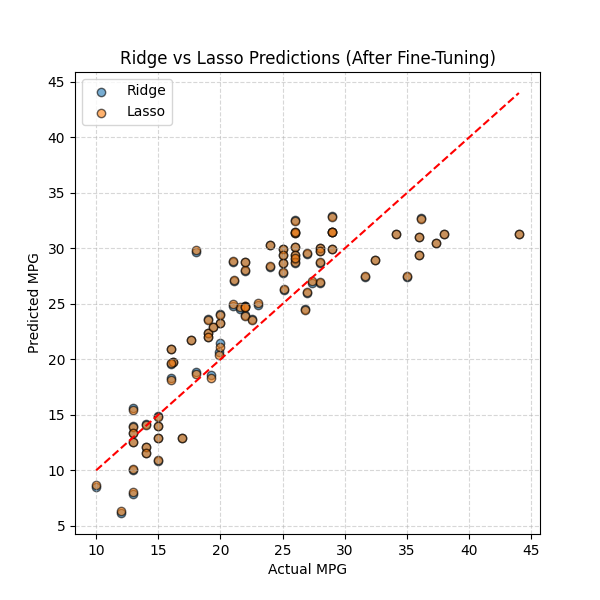
\includegraphics[width=0.75\columnwidth]{../models/ridge_vs_lasso_after_finetuning.png}
    \caption{Sammenligning af forudsigelser mellem Ridge og Lasso efter finjustering. De fleste datapunkter ligger tæt på den stiplede linje, hvilket indikerer høj præcision i forudsigelsen af MPG.}
    \label{fig:regression}
\end{figure}


